In this section we present the \emph{resource allocation}. For each
member of the team we will associate the tasks, as defined in the
previous section, to be executed with reference to the available time
of each team member. Since all team members contributed to the project
playing different roles in the context of the software development
cycle we will specify that role time by time.


\subsection{Resource allocation}

For the task we actually performed the hours specified are the real
ones, for the others we estimated a reasonable allocation of time
also according to our availability being university students. Moreover,
according to our previous experiences, we qualified the implementation
and the testing phases as the most time consuming. 

The following table shows for each task the role played by the team
member and the hours allocated; the attribute ``Units'', as commonly
used in resource planning is the percentage ratio between the used
hours and the allocated hours computed as the duration in days times
8 hours per day. As emerges from the table those values are by far
lower than 50\% because of our university activity.

\begin{landscape}

\begin{tabular}{l|>{\raggedright}p{6.5cm}|>{\centering}m{1.5cm}|>{\centering}p{3.5cm}|c|c|>{\centering}p{3.5cm}|c|c}
\hline 
\multirow{2}{*}{\emph{Task id}} & \multirow{2}{6.5cm}{\emph{Name}} & \multirow{2}{1.5cm}{\emph{Duration}} & \multicolumn{3}{c|}{\textbf{\emph{Riccardo Mologni}}} & \multicolumn{3}{c}{\textbf{\emph{Alberto Maria Metelli}}}\tabularnewline
\cline{4-9} 
 &  &  & \emph{Role} & \textit{Hours} & \emph{Units} & \textit{Role} & \emph{Hours} & \emph{Units}\tabularnewline
\hline 
\hline 
T1 & \textbf{Project planning} & 10 & {\small{}Project Manager} & 10 & 12,5\% & {\small{}Project Manager} & 10 & 12,5\%\tabularnewline
\hline 
T11 & {\footnotesize{}Project scheduling} & 7 & {\small{}Project Manager} & 5 & 8,9\% & {\small{}Project Manager} & 3 & 5,4\%\tabularnewline
\hline 
T12 & {\footnotesize{}Resource allocation} & 3 & {\small{}Project Manager} & 3 & 12,5\% & {\small{}Project Manager} & 3 & 12,5\%\tabularnewline
\hline 
T13 & {\footnotesize{}Risk planning} & 8 & {\small{}Project Manager} & 2 & 3,1\% & {\small{}Project Manager} & 4 & 6,3\%\tabularnewline
\hline 
T2 & \textbf{Requirement analysis and specification} & 13 & {\small{}Analyst} & 33 & 31,7\% & {\small{}Analyst} & 33 & 31,7\%\tabularnewline
\hline 
T21 & {\footnotesize{}Requirement engineering} & 5 & {\small{}Requirements engineer} & 12 & 30,0\% & {\small{}Requirements engineer} & 12 & 30,0\%\tabularnewline
\hline 
T22 & {\footnotesize{}Use case design} & 8 & {\small{}Analyst} & 15 & 23,4\% & {\small{}Analyst} & 11 & 17,2\%\tabularnewline
\hline 
T23 & {\footnotesize{}High level data design} & 3 & {\small{}Analyst} & 3 & 12,5\% & {\small{}Analyst} & 3 & 12,5\%\tabularnewline
\hline 
T24 & {\footnotesize{}Alloy modeling} & 3 & {\small{}Analyst} & 3 & 12,5\% & {\small{}Analyst} & 7 & 29,2\%\tabularnewline
\hline 
T3 & \textbf{Acceptance test plan design} & 7 & {\small{}Analyst} & 8 & 14,3\% & {\small{}Analyst} & 8 & 14,3\%\tabularnewline
\hline 
T4 & \textbf{Design} & 20 & {\small{}Software Architect} & 30 & 18,8\% & {\small{}Software Architect} & 35 & 21,9\%\tabularnewline
\hline 
T41 & {\footnotesize{}Architectural design} & 20 & {\small{}Software Architect} & 15 & 9,4\% & {\small{}Software Architect} & 15 & 9,4\%\tabularnewline
\hline 
T42 & {\footnotesize{}Algorithm design} & 15 & {\small{}Software Architect} & 7 & 5,8\% & {\small{}Software Architect} & 15 & 12,5\%\tabularnewline
\hline 
T43 & {\footnotesize{}User interface design} & 5 & {\small{}Software Architect} & 8 & 20,0\% & {\small{}Software Architect} & 5 & 12,5\%\tabularnewline
\hline 
T5 & \textbf{Unit test plan design} & 7 & {\small{}Analyst} & 13 & 23,2\% & {\small{}Analyst} & 13 & 23,2\%\tabularnewline
\hline 
T6 & \textbf{Integration test plan design} & 11 & {\small{}Analyst} & 12 & 13,6\% & {\small{}Analyst} & 12 & 13,6\%\tabularnewline
\hline 
T7 & \textbf{Implementation} & 65 & {\small{}Developer} & 260 & 50,0\% & {\small{}Developer} & 260 & 50,0\%\tabularnewline
\hline 
T71 & {\footnotesize{}Components implementation} & 65 & {\small{}Developer} & 200 & 38,5\% & {\small{}Developer} & 200 & 38,5\%\tabularnewline
\hline 
T72 & {\footnotesize{}Subsystem implementation} & 20 & {\small{}Developer} & 60 & 37,5\% & {\small{}Developer} & 60 & 37,5\%\tabularnewline
\hline 
T8 & \textbf{Code Ispection} & 13 & {\small{}Ispector} & 15 & 14,4\% & {\small{}Ispector} & 18 & 17,3\%\tabularnewline
\hline 
T81 & {\footnotesize{}Manual inspection} & 9 & {\small{}Ispector} & 13 & 18,1\% & {\small{}Ispector} & 13 & 18,1\%\tabularnewline
\hline 
T82 & {\footnotesize{}Automated code inspection} & 4 & {\small{}Ispector} & 2 & 6,3\% & {\small{}Ispector} & 5 & 15,6\%\tabularnewline
\hline 
T9 & \textbf{Testing} & 26 & {\small{}Tester} & 86 & 41,3\% & {\small{}Tester} & 86 & 41,3\%\tabularnewline
\hline 
T91 & {\footnotesize{}Unit testing} & 12 & {\small{}Tester} & 45 & 46,9\% & {\small{}Tester} & 45 & 46,9\%\tabularnewline
\hline 
T92 & {\footnotesize{}Integration testing} & 6 & {\small{}Tester} & 25 & 52,1\% & {\small{}Tester} & 25 & 52,1\%\tabularnewline
\hline 
T93 & {\footnotesize{}System and performance testing} & 2 & {\small{}Tester} & 6 & 37,5\% & {\small{}Tester} & 6 & 37,5\%\tabularnewline
\hline 
T94 & {\footnotesize{}Acceptance testing} & 6 & {\small{}Tester} & 10 & 20,8\% & {\small{}Tester} & 10 & 20,8\%\tabularnewline
\hline 
T10 & \textbf{Deployment} & 4 & {\small{}Installer} & 15 & 46,9\% & {\small{}Installer} & 15 & 46,9\%\tabularnewline
\hline 
\end{tabular}

\end{landscape}

\begin{landscape}

The following is the same table in which just macro tasks are represented.

\medskip{}


\begin{tabular}{l|>{\raggedright}p{6.5cm}|>{\centering}m{1.5cm}|>{\centering}p{3.5cm}|c|c|>{\centering}p{3.5cm}|c|c}
\hline 
\multirow{2}{*}{\emph{Task id}} & \multirow{2}{6.5cm}{\emph{Name}} & \multirow{2}{1.5cm}{\emph{Duration}} & \multicolumn{3}{c|}{\textbf{\emph{Riccardo Mologni}}} & \multicolumn{3}{c}{\textbf{\emph{Alberto Maria Metelli}}}\tabularnewline
\cline{4-9} 
 &  &  & \emph{Role} & \textit{Hours} & \emph{Units} & \textit{Role} & \emph{Hours} & \emph{Units}\tabularnewline
\hline 
\hline 
T1 & Project planning & 10 & {\small{}Project Manager} & 10 & 12,5\% & {\small{}Project Manager} & 10 & 12,5\%\tabularnewline
\hline 
T2 & Requirement analysis and specification & 13 & {\small{}Analyst} & 33 & 31,7\% & {\small{}Analyst} & 33 & 31,7\%\tabularnewline
\hline 
T3 & Acceptance test plan design & 7 & {\small{}Analyst} & 8 & 14,3\% & {\small{}Analyst} & 8 & 14,3\%\tabularnewline
\hline 
T4 & Design & 20 & {\small{}Software Architect} & 30 & 18,8\% & {\small{}Software Architect} & 35 & 21,9\%\tabularnewline
\hline 
T5 & Unit test plan design & 7 & {\small{}Analyst} & 13 & 23,2\% & {\small{}Analyst} & 13 & 23,2\%\tabularnewline
\hline 
T6 & Integration test plan design & 11 & {\small{}Analyst} & 12 & 13,6\% & {\small{}Analyst} & 12 & 13,6\%\tabularnewline
\hline 
T7 & Implementation & 65 & {\small{}Developer} & 260 & 50,0\% & {\small{}Developer} & 260 & 50,0\%\tabularnewline
\hline 
T8 & Code Ispection & 13 & {\small{}Ispector} & 15 & 14,4\% & {\small{}Ispector} & 18 & 17,3\%\tabularnewline
\hline 
T9 & Testing & 26 & {\small{}Tester} & 86 & 41,3\% & {\small{}Tester} & 86 & 41,3\%\tabularnewline
\hline 
T10 & Deployment & 4 & {\small{}Installer} & 15 & 46,9\% & {\small{}Installer} & 15 & 46,9\%\tabularnewline
\hline 
\end{tabular}

\end{landscape}


\subsection{Cumulative data}

In this subsection we report some cumulative data derived from the
previous table. We want to make a clear distinction between real deta
referred to the task we actually performed and estimated data.


\subsubsection{Estimated data}
\begin{itemize}
\item \emph{Total duration}: 176 days (1408 h)
\item \emph{Total working hours}

\begin{itemize}
\item Riccardo Mologni: 482 h
\item Alberto Maria Metelli: 490 h
\end{itemize}
\item \emph{Working hours per day}

\begin{itemize}
\item Riccardo Mologni: 2,72 h/day
\item Alberto Maria Metelli: 2,78 h/day
\end{itemize}
\item \emph{Units}

\begin{itemize}
\item Riccardo Mologni: 34,2\%
\item Alberto Maria Metelli: 34,8\%
\end{itemize}
\end{itemize}

\subsubsection{Real data}
\begin{itemize}
\item \emph{Total duration}: 67 days (536 h)
\item \emph{Total working hours}

\begin{itemize}
\item Riccardo Mologni: 100 h
\item Alberto Maria Metelli: 108 h
\end{itemize}
\item \emph{Working hours per day}

\begin{itemize}
\item Riccardo Mologni: 0,57 h/day
\item Alberto Maria Metelli: 0,61 h/day
\end{itemize}
\item \emph{Units}

\begin{itemize}
\item Riccardo Mologni: 18,7\%
\item Alberto Maria Metelli: 20,1\%
\end{itemize}
\end{itemize}
\begin{landscape}

\newgeometry{left=2.5cm,bottom=0cm,top=2.5cm,right=-7cm}


\subsection{Resource allocation chart}

\medskip{}


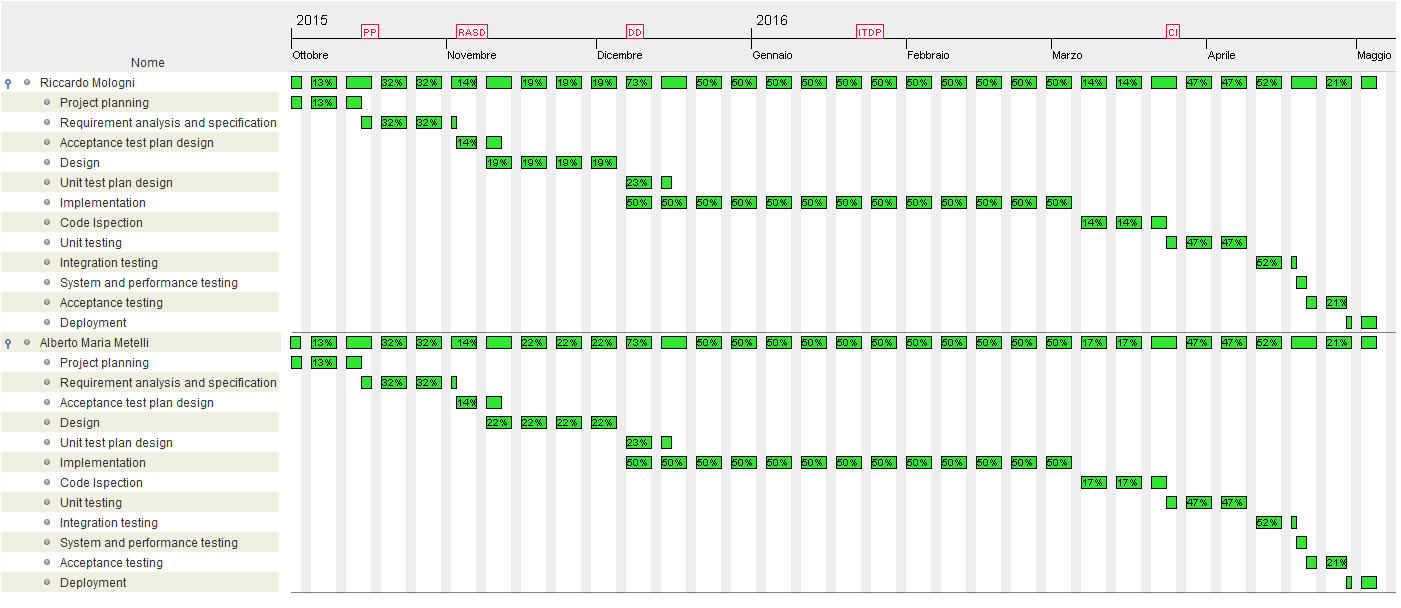
\includegraphics[scale=0.7]{resources/resources}

\restoregeometry

\end{landscape}
